% NOTE - this is only a template without real arguments
\begin{entry}{Measurement processor and Log Early Implementation}{Sep 2, 2021}
    \objective 
    
    Determine a data scheme for internal data (I.E. grid states and association data passed to the GO and logger.)
    Implement MCOutputLog
    Run a simulation and get output logs

    \outline

    \begin{itemize}
        \item Select data scheme (DICT OF DICTS)
        \item Add processing to EDMMeasurementProcessor
        \item Add accessor function to EDMMeasurementProcessor
        \item Write MCOutputLog
        \item Add accessor-logger routine to timekeeper
        \item Add log writing routine to timekeeper
        \item Add file closeout function to timekeeper closeout
        \item Test

    \end{itemize}

    \procedures
    
    See outline. Not much to add here. I'll come up with the test as I go along (see observations) since this is a
    pretty simple communication feedthrough in spite of how crucial it is to the system.

    \parameters
    
    N/A

    \observations
    


    \data
    
    N/A

    \results
    


\end{entry}


%\begin{entry}{CMake Error running EGOT-DCM Dockerfile}{Dec 02, 2020}
%    \objective
%
%    Determine the cause of the CMake error while running the dockerfile and modify file to get it to successfully build.
%
%    \outline
%
%    \begin{itemize}
%        \item Try running to see if it was just Lorry or a machine issue.
%        \item If it is a machine issue, modify configurations to ensure interoperability.
%        \item If I get the error track down its cause and modify dockerfile to fix.
%        \item Repeat until all builds are successful.
%    \end{itemize}
%
%    \procedures
%
%    \begin{itemize}
%        \item \mint{console}|git clone https://github.com/EGoT-DCS-SunSpec-Modbus|
%        \item \mint{console}|docker build -f Dockerfile.buster -t egot-dcs .|
%        \item \mint{console}|docker container run -i egot-dcs|
%    \end{itemize}
%
%    \observations
%
%    \begin{error}{Cmake Error: No CMAKE\_CXX\_COMPILER found}
%        \begin{figure}[H]
%            \centering
%            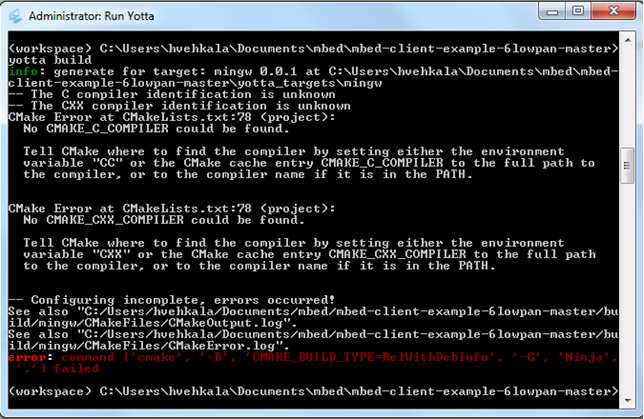
\includegraphics[height=4in]{Fall2020/Figures/cmake_error.png}
%        \end{figure}
%
%        Solution: what you need to do found at \cite{CMAKE-Forum}
%    \end{error}
%
%    \results
%
%    Short: No.
%
%    Long: Well...
%
%
%\end{entry}